\documentclass[11pt,a4paper]{article}
\usepackage[utf8]{inputenc}
\usepackage[T1]{fontenc}
\usepackage[provide=*,spanish]{babel}
\usepackage{lmodern,microtype}
\usepackage[a4paper,margin=1.8cm,top=1.6cm,bottom=1.7cm]{geometry}
\usepackage{booktabs,tabularx,longtable,array,xcolor,amsmath,graphicx}
\usepackage[hidelinks]{hyperref}
\usepackage{titlesec,fancyhdr}
\definecolor{azul}{HTML}{173B56}
\titleformat{\section}{\large\bfseries\color{azul}}{\thesection.}{0.5em}{}
\titlespacing*{\section}{0pt}{10pt}{7pt}
\setlength{\parindent}{0pt}
\setlength{\parskip}{7pt}
\setlength{\emergencystretch}{2em}
\pagestyle{fancy}\fancyhf{}\fancyfoot[R]{\small\thepage}
\renewcommand{\headrulewidth}{0pt}
\newcolumntype{Y}{>{\raggedright\arraybackslash}X}
\begin{document}
{\LARGE\bfseries\color{azul} Informe ejecutivo}\par
{\small Aprendizaje no supervisado aplicado a datos comerciales y operativos de DataCo}

\section{Problema, descripción del dataset y decisiones de preprocesamiento}
Los datos comerciales integran información sobre clientes, productos, ventas, descuentos, rentabilidad y envíos. Su volumen y las relaciones entre variables dificultan reconocer perfiles transaccionales, identificar factores latentes y caracterizar observaciones atípicas mediante estadísticas descriptivas únicamente. Además, transacciones con ventas similares pueden presentar márgenes de rentabilidad diferentes, mientras que un comportamiento inusual puede estar asociado tanto con resultados favorables como desfavorables para el negocio. Por ello, este estudio explora diferentes enfoques de aprendizaje no supervisado para responder la siguiente pregunta:

\begingroup\leftskip=10pt\rightskip=10pt
\textbf{¿Qué estructuras, relaciones y patrones latentes pueden identificarse en los datos comerciales y operativos de pedidos mediante diferentes enfoques de aprendizaje no supervisado, y en qué medida permiten caracterizar perfiles comerciales, explorar afinidades entre clientes y productos e identificar comportamientos atípicos?}\par
\endgroup

Se utilizó el dataset de cadena de suministro de \textbf{DataCo}, compuesto originalmente por \textbf{180.519 registros y 53 variables} comerciales y operativas. La unidad de análisis corresponde a un ítem de pedido; por tanto, varios registros pueden pertenecer a una misma orden. El conjunto incluye atributos de productos, clientes, ubicación geográfica, ventas, descuentos, beneficios y tiempos de envío.

El preprocesamiento eliminó columnas con información insuficiente, como \textit{Product Description}, completamente vacía, y \textit{Order Zipcode}, con aproximadamente 86,24\% de valores faltantes. También se descartaron columnas constantes, atributos redundantes, identificadores de pedidos e ítems y datos personales innecesarios para los objetivos del estudio. Se conservaron los identificadores de clientes y productos para analizar sus interacciones, se extrajo \textit{Order Month} de la fecha del pedido y se mantuvieron valores negativos de rentabilidad por representar pérdidas comercialmente posibles. No se encontraron filas duplicadas ni se eliminaron observaciones.

El conjunto procesado conservó \textbf{180.519 registros y 33 variables}. La mayoría de los modelos numéricos utilizó diez características relacionadas con duración real y programada del envío, beneficio, ventas, descuentos, rentabilidad, cantidad y precio. GMM empleó un subconjunto de cuatro variables para construir perfiles interpretables, mientras que el recomendador utilizó interacciones entre clientes y productos.

\section{Metodología, hiperparámetros y criterios de validación}
La metodología se organizó por objetivos: identificar perfiles probabilísticos, extraer representaciones latentes, explorar relaciones no lineales, generar recomendaciones y detectar observaciones atípicas. Los modelos se evaluaron con criterios específicos para cada tarea, combinando desempeño cuantitativo, estabilidad e interpretación comercial. La selección buscó equilibrar calidad de representación y complejidad, sin asumir que una única técnica fuera superior para todos los objetivos.

\begingroup
\fontsize{9}{10.8}\selectfont
\setlength{\tabcolsep}{5pt}
\renewcommand{\arraystretch}{1.12}
\setlength{\LTpre}{0pt}
\setlength{\LTpost}{5pt}
\begin{longtable}{@{}>{\raggedright\arraybackslash}p{2.55cm}*{2}{>{\raggedright\arraybackslash}p{\dimexpr(\textwidth-2.55cm-4\tabcolsep)/2\relax}}@{}}
\toprule
\textbf{Objetivo y modelos} & \textbf{Configuración seleccionada} & \textbf{Selección y validación}\\
\midrule
\endfirsthead
\toprule
\textbf{Objetivo y modelos} & \textbf{Configuración seleccionada} & \textbf{Selección y validación}\\
\midrule
\endhead
\midrule
\endfoot
\bottomrule
\endlastfoot
Perfiles: GMM & Cuatro componentes, covarianza diagonal y diez inicializaciones. Ventas, tasa de descuento, ratio de beneficio y cantidad. & 32 configuraciones; AIC, BIC, log-verosimilitud, silhouette, Davies--Bouldin y Calinski--Harabasz. Interpretabilidad y ARI entre diez semillas.\\[4pt]
Reducción: SVD, PCA y PPCA & Cinco componentes por método, explorando entre uno y nueve. & MSE, error relativo de Frobenius, energía o varianza retenida, estabilidad del subespacio con diez remuestreos bootstrap e interpretación. PPCA: log-verosimilitud.\\[4pt]
Factores: FA e ICA & FA: cinco factores con rotación varimax. ICA: cinco componentes y blanqueamiento de varianza unitaria. & Reconstrucción, energía recuperada, estabilidad bootstrap, concentración de coeficientes, convergencia e interpretación de cargas.\\[4pt]
Recomendaciones: SVD & Dos factores latentes y listas de diez productos; comparación con una baseline de popularidad. & HitRate@10 y NDCG@10 sobre interacciones reservadas para validación y prueba.\\[4pt]
Visualización: t-SNE y UMAP & Dos dimensiones. t-SNE: perplexity=30. UMAP: n\_neighbors=30 y min\_dist=0,1. & Trustworthiness y overlap para $k=2,5,10,30,50$; Spearman global de distancias y estabilidad de vecinos entre diez semillas.\\[4pt]
Anomalías: PCA, ICA y Mahalanobis & PCA e ICA: cinco componentes. ICA: KDE gaussiana, bandwidth=0,3 y 5.000 observaciones. Mahalanobis: covarianza Ledoit--Wolf. & Scores $T^2$, SPE, NLL y distancia cuadrática; umbrales de entrenamiento y comparación descriptiva de observaciones señaladas y no señaladas.\\[4pt]
Anomalías: LOF e IF & LOF: veinte vecinos. IF final: cuatrocientos árboles y 1.024 observaciones por árbol. & Sensibilidad de hiperparámetros, Spearman de scores y Jaccard del 1\% más extremo. LOF: remuestreo; IF: semillas.\\[4pt]
Redes: AE y VAE & AE: cinco dimensiones, 64 neuronas ocultas, learning rate=0,001 y lotes de 128. VAE: cinco dimensiones, 64 neuronas ocultas, $\beta=0{,}001$, learning rate=0,001 y lotes de 256. & AE: MSE de validación, CKA latente y RMSE entre reconstrucciones. VAE: MSE+$\beta\cdot$KL. Adam, detención temprana y estabilidad entre diez semillas.\\
Asociaciones: Apriori & Soporte mínimo de 0,05; confianza mínima de 0,50 y filtro lift mayor que 1. Matriz binaria cliente--producto. & Soporte, confianza y lift sobre historiales de compra; no establecen secuencia temporal ni efecto causal.\\
\end{longtable}
\endgroup

\begingroup\fontsize{10}{12}\selectfont
GMM utilizó una división de \textbf{80\%/20\%} para entrenamiento y validación. Los métodos de reducción dimensional y análisis factorial emplearon \textbf{70\%/15\%/15\%}, y los modelos de anomalías y las redes neuronales, \textbf{60\%/20\%/20\%} para entrenamiento, validación y prueba. El recomendador reservó interacciones entre clientes y productos; t-SNE y UMAP evaluaron hiperparámetros sobre \textbf{30.000 observaciones}. El escalamiento se ajustó con entrenamiento cuando existía esta partición: SVD sin centrado y los demás modelos numéricos con estandarización centrada. t-SNE y UMAP ajustaron el escalamiento sobre los datos completos para su análisis exploratorio.

Las anomalías se señalaron con los percentiles \textbf{95 y 99 de los scores de entrenamiento} ($\alpha=0{,}05$ y $\alpha=0{,}01$). Estos criterios permiten explorar conjuntos de distinta amplitud, sin confirmar errores o amenazas. Al no disponer de etiquetas verificadas, se evaluaron estabilidad, sensibilidad e interpretación descriptiva, sin estimar exactitud ni tasas de falsos positivos y negativos.\par
\endgroup

\section{Resultados comparativos e interpretación}
\textbf{Perfiles comerciales y representaciones latentes.} GMM identificó compras de un artículo generalmente rentables (53\%), compras pequeñas de dos artículos (10\%), transacciones con pérdidas (5,8\%) y compras de varios artículos mayoritariamente rentables (30\%). SVD, PCA y PPCA recuperaron temas similares de valor transaccional, rentabilidad, descuentos, envío y cantidad--precio; PCA y PPCA fueron especialmente próximos, mientras que SVD mezcló más algunas contribuciones al no centrar los datos. FA e ICA recuperaron temas semejantes, pero con ejes y ponderaciones parcialmente diferentes de PCA. Todas estas representaciones admitieron interpretaciones comerciales descriptivas, sin demostrar causalidad.


\begingroup
\fontsize{8.3}{10}\selectfont
\setlength{\tabcolsep}{3pt}\renewcommand{\arraystretch}{1.18}
\setlength{\LTpre}{3pt}\setlength{\LTpost}{4pt}
\begin{longtable}{@{}>{\raggedright\arraybackslash}p{1.1cm}*{5}{>{\raggedright\arraybackslash}p{\dimexpr(\textwidth-1.1cm-10\tabcolsep)/5\relax}}@{}}
\toprule
\textbf{Modelo} & \textbf{Dimensión 1} & \textbf{Dimensión 2} & \textbf{Dimensión 3} & \textbf{Dimensión 4} & \textbf{Dimensión 5}\\
\midrule
\endfirsthead
\toprule
\textbf{Modelo} & \textbf{Dimensión 1} & \textbf{Dimensión 2} & \textbf{Dimensión 3} & \textbf{Dimensión 4} & \textbf{Dimensión 5}\\
\midrule
\endhead
\midrule
\endfoot
\bottomrule
\endlastfoot
SVD & Envíos largos y mayor actividad transaccional. & Mayor valor y precio, con envíos cortos y menor cantidad. & Mayor beneficio y proporción de ganancia. & Más descuentos, con envíos cortos. & Más unidades de productos económicos.\\[3pt]
PCA & Ventas y precios altos, con mayores descuentos absolutos. & Mayor beneficio y proporción de ganancia. & Mayor duración real y programada del envío. & Más descuentos, con ventas y precios relativamente bajos. & Más unidades, menor precio y tasa de descuento.\\[3pt]
PPCA & Ventas y precios altos. & Mayor beneficio y proporción de ganancia. & Mayor duración real y programada del envío. & Más descuentos, con menor precio y venta por cliente. & Más unidades, menor precio y tasa de descuento.\\[3pt]
FA & Mayor valor transaccional y precio. & Mayor intensidad de descuentos. & Mayor precio y menor cantidad. & Menor beneficio y proporción de ganancia. & Envíos reales y programados más cortos.\\[3pt]
ICA & Mayor intensidad de descuentos. & Menor beneficio y proporción de ganancia. & Mayor precio y menor cantidad. & Envíos reales y programados más largos. & Mayor valor, precio y descuento absoluto.\\[3pt]
AE & Más descuentos, envíos largos y mayor precio. & Más unidades, menor precio y envíos más largos. & Más unidades, menor precio y envíos más cortos. & Menor cantidad y menores ventas. & Mayor rentabilidad y envíos más cortos.\\
\end{longtable}\par
\textit{Lectura:} cada celda describe el patrón asociado a valores altos de esa dimensión en el modelo seleccionado. El orden y el signo de los ejes pueden cambiar entre modelos; no son categorías de órdenes. En AE se observa qué variables aumentan o disminuyen junto con cada dimensión, sin atribuirles un efecto causal ni una contribución exacta a la red.
\endgroup

\begin{center}
\begin{minipage}{\linewidth}\centering
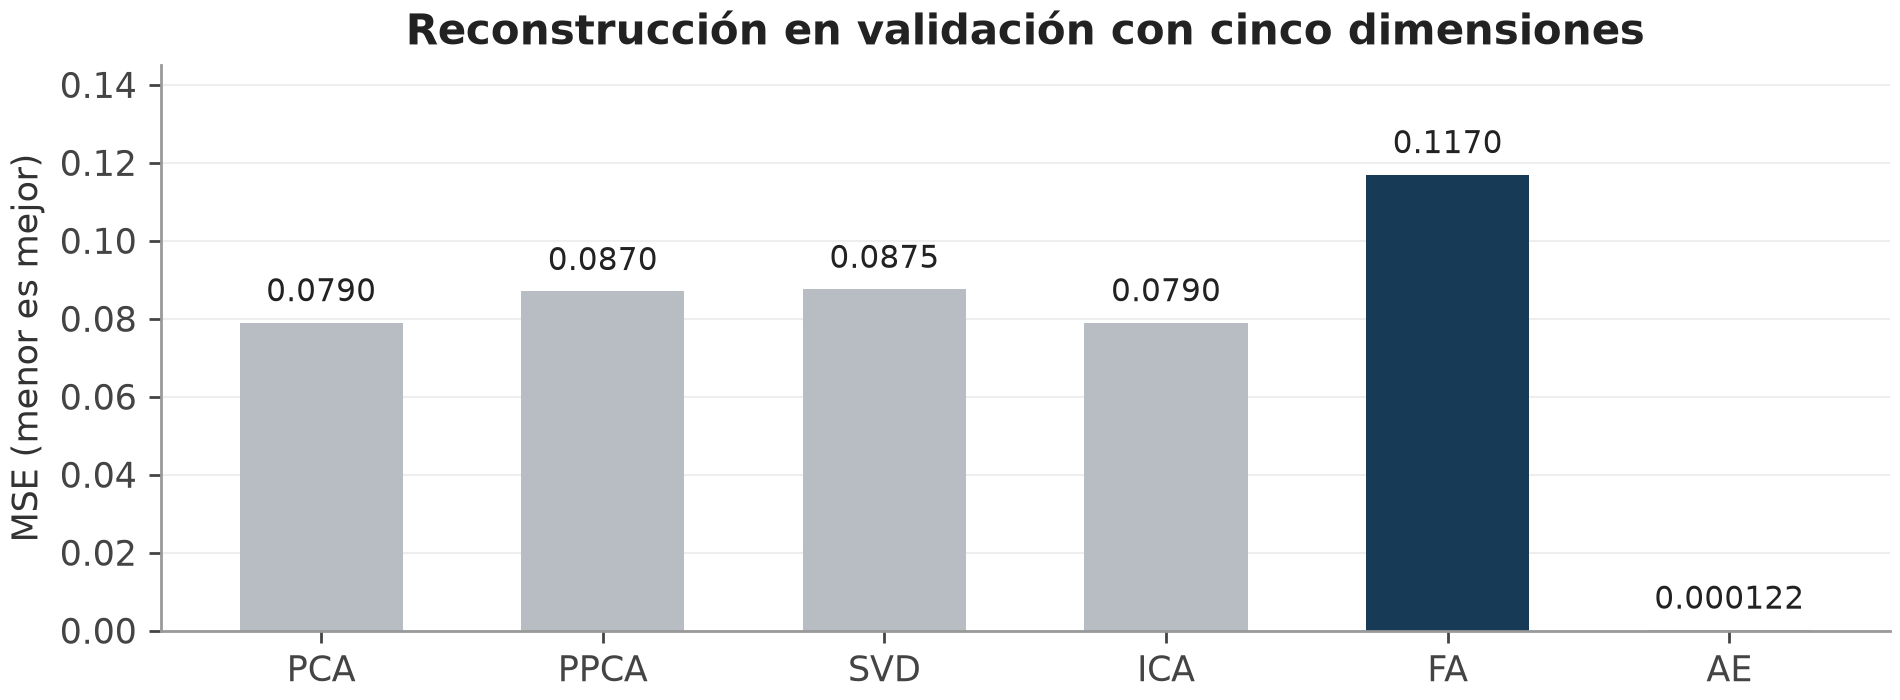
\includegraphics[width=0.94\linewidth]{figuras/05_reconstruccion_todos_modelos.png}\par
{\footnotesize\textbf{Figura 1.} Error de reconstrucción: se resalta FA por presentar el mayor MSE, no el mejor desempeño. Todos usan cinco dimensiones; SVD no centra y AE emplea otra partición (60/20/20 frente a 70/15/15). La comparación es descriptiva, no una clasificación controlada de superioridad.}
\end{minipage}
\end{center}

El AE compartió temas con los métodos lineales, pero los combinó de otra forma: AE1 vinculó descuentos y envíos largos; AE2--AE3, cantidad y menor precio; AE4, menor cantidad y ventas; y AE5, rentabilidad y envíos cortos. Su interpretación corresponde al modelo seleccionado y mostró sensibilidad a la semilla.

\textbf{Recomendación, visualización y asociaciones.} La popularidad superó al SVD de dos factores en prueba: HitRate@10 de 0,8507 frente a 0,8298 y NDCG@10 de 0,6572 frente a 0,5810. Los veinte productos más populares concentraron alrededor del 82\% de interacciones. t-SNE preservó mejor los vecinos próximos (overlap@10 cercano a 0,74), mientras UMAP conservó mejor el orden global de distancias que el t-SNE seleccionado (Spearman de 0,315 frente a 0,13), aunque ambas correlaciones fueron limitadas. Shipping Mode mostró la segmentación más clara; productos y categorías presentaron concentraciones locales. Apriori produjo 511 conjuntos frecuentes y 9.206 reglas; las diez primeras repartieron los mismos nueve productos, con soporte de 6,18\%, confianza de 50--58\% y lift de 2,55--2,60. Estas asociaciones pueden orientar campañas, pero no prueban ventas adicionales.

\textbf{Ejemplo documentado: regla 9205.} $A\Rightarrow B$, con nombres abreviados: $A$ reúne Nike Free, zapatillas Under Armour infantiles, bicicleta Diamondback Serene y kayak Pelican Sunstream; $B$ reúne Perfect Fitness Rip Deck, botines Nike CJ Elite, polo Nike Dri-FIT, caja de seguridad Field \& Stream y chaleco O'Brien. Su soporte es \textbf{6,18\%}: esa proporción de clientes compró los nueve productos. La confianza es \textbf{54,44\%}: entre quienes compraron todos los productos de $A$, ese porcentaje también compró todos los de $B$. El lift de \textbf{2,60} indica que adquirir el conjunto completo $B$ fue 2,60 veces más frecuente entre compradores de $A$ que entre clientes en general. No establece secuencia temporal ni causalidad.

\begin{center}
\begin{minipage}{\linewidth}\centering
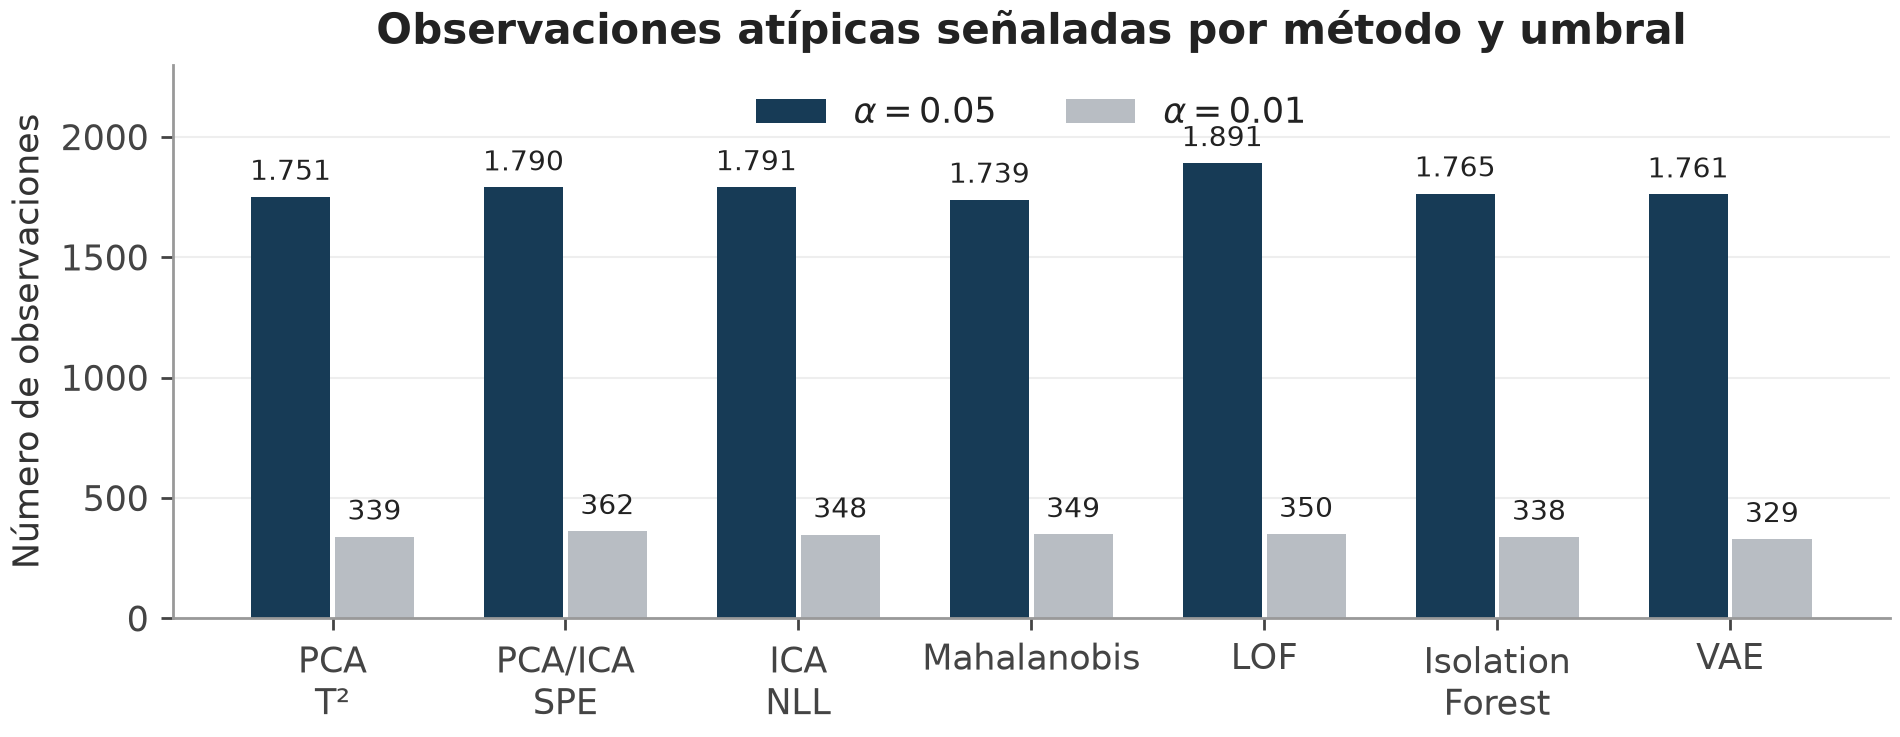
\includegraphics[width=0.94\linewidth]{figuras/06_conteo_anomalias_metodos.png}\par
{\footnotesize\textbf{Figura 2.} Validación: 36.104 registros; umbrales derivados del entrenamiento. PCA e ICA--SPE se agrupan por coincidir sus resultados. Los conteos se solapan y no deben sumarse.}
\end{minipage}
\end{center}

\textbf{Atipicidad y selección del umbral.} Para cada umbral, los métodos señalaron cantidades parecidas: 1.739--1.891 registros al 5\% y 329--362 al 1\%, incluyendo VAE; esto no implica que seleccionaran los mismos casos ni que tuvieran igual precisión. Las observaciones incluyeron pérdidas, ganancias elevadas y combinaciones inusuales de ventas, descuentos, cantidades y envío. Por ello, ser atípico no implica perjudicar al negocio, y una ganancia alta tampoco descarta otros problemas operativos.

No se dispone de etiquetas verificadas de anomalía. Elevar el umbral reduce la cantidad de detecciones y puede aumentar los falsos negativos; reducirlo amplía las detecciones y puede aumentar los falsos positivos. Estas tasas no se midieron y los valores de $\alpha$ no las representan. Se recomienda $\alpha=0,05$ como criterio \emph{exploratorio}: permite revisar una mayor diversidad potencial de casos, incluidos algunos menos extremos que con $\alpha=0,01$, sin demostrar superioridad en exactitud.


\section{Conclusiones, limitaciones, sesgos y trabajo futuro}
\textbf{Conclusiones.} Los enfoques fueron complementarios: GMM permitió caracterizar perfiles probabilísticos; las representaciones latentes resumieron dimensiones comerciales interpretables; y t-SNE y UMAP facilitaron explorar similitudes. La reconstrucción, la estabilidad y la interpretabilidad deben evaluarse por separado. En recomendación, la baseline de popularidad superó al SVD implementado; las reglas aportaron asociaciones exploratorias para venta cruzada. Las anomalías representan atipicidad estadística, no daño confirmado, por lo que deben priorizarse según objetivos del negocio.

\textbf{Limitaciones y sesgos.} La ausencia de etiquetas impidió medir exactitud y errores de detección. Los resultados dependen de variables, escalamiento, parámetros, semillas y umbrales. En t-SNE y UMAP, cambiar las características puede modificar vecinos y agrupaciones; las categorías usadas como colores solo contextualizan el mapa. Variables monetarias relacionadas pueden reforzar patrones similares. La popularidad, la actividad de los clientes y la cobertura desigual del dataset condicionan recomendaciones y reglas; estas últimas describen historiales, sin establecer secuencia ni causalidad. Los factores latentes son interpretaciones descriptivas y las dimensiones de AE mostraron sensibilidad entre ejecuciones.

\textbf{Trabajo futuro.} Se propone explicar las contribuciones individuales a las anomalías, distinguir resultados beneficiosos y adversos y contextualizarlos por región, cliente y producto. También conviene validar estabilidad temporal, evaluar diversidad y cobertura del recomendador, reducir la redundancia de reglas, complementar el análisis de asociaciones con FP-Growth y contrastar promociones mediante experimentos que midan ventas incrementales y rentabilidad.

\end{document}
